\documentclass[12pt]{article}

\usepackage[utf8]{inputenc}
\usepackage[russian]{babel}
\usepackage[T2A]{fontenc}
\usepackage{textcomp}
\usepackage{a4wide}
\usepackage{amsmath, amssymb}
\usepackage{graphicx}
\usepackage{wrapfig}
\usepackage{caption}
\usepackage{subfig}
\usepackage{listings}
\usepackage{hyperref}
% \usepackage{fontspec}
\usepackage{pgfplots}
\usepackage{tikz}
\usepackage{amsthm}
\usepackage{pgf,pgfarrows,pgfnodes}
\usepackage{pgf}
\lstset{
	language=Python,
	basicstyle=\ttfamily\small,
	otherkeywords={self},                   
}
\hypersetup{
    colorlinks = true,
    urlcolor = blue
}

\begin{document}
	
\renewcommand{\contentsname}{\centerline{\bf Contents}}
\renewcommand{\figurename}{Fig.}
\renewcommand{\refname}{\centerline{\bf Literature}}

\newcommand{\GP}{\mathcal{GP}}
\newcommand{\E}{\mathbb{E}}
\newcommand{\R}{\mathbb{R}}
\newcommand{\N}{\mathcal{N}}
\newcommand{\bigO}{\mathcal{O}}
\newcommand{\cov}{\mbox{cov}}
\newcommand{\Nystrom}{Nystr\"{o}m }
\newcommand{\KL}[2]{\mbox{KL}\left(#1\mbox{ || }#2\right)}
\newcommand{\tr}{\mbox{tr}}
\newcommand{\derivative}[2]{\frac{\partial #1}{\partial #2}}
\newcommand{\sndderivative}[3]{\frac{\partial^2 #1}{\partial #2 \partial #3}}

\newlength{\arrayrulewidthOriginal}
\newcommand{\Cline}[2]{%
  \noalign{\global\setlength{\arrayrulewidthOriginal}{\arrayrulewidth}}%
  \noalign{\global\setlength{\arrayrulewidth}{#1}}\cline{#2}%
  \noalign{\global\setlength{\arrayrulewidth}{\arrayrulewidthOriginal}}}

\newtheorem{definition}{Definition}
\newtheorem{theorem}{Theorem}

\begin{titlepage}
  \centering
  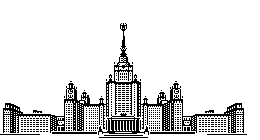
\includegraphics{pictures/msu.jpg}\par\vspace{1cm}
  {\scshape lomonosov Moscow State University\\ faculty of computational mathematics and cybernetics\\ chair of mathematical methods of forecasting \par}
  \vspace{2cm}
  {\scshape\large Izmailov Pavel\par}
  \vspace{1cm}
  {\LARGE\bfseries Gaussian Processes for Machine Learning\par}
  \vspace{1.5cm}
  {\scshape COURSE WORK\par}
  \vfill

  \raggedleft
  
  {\bf Scientific advisors:}\par
  % д.ф-м.н., профессор\par
  D. P. Vetrov\\
  D. A. Kropotov
  
  \vfill
  {\center\large Moscow, 2016\par}
\end{titlepage}

\pagebreak
{\hypersetup{linkcolor=black}
	\tableofcontents
}
% \tableofcontents
\pagebreak
\centerline{\bf Abstract}

Gaussian processes provide an elegant and effective approach to learning in kernel machines. This approach leads to a highly interpretable model and allows using the bayesian framework for model adaptation and incorporating the prior knowledge about the problem. Unfortunately, the standard methods for GP-regression and GP-classification scale as $\bigO(n^3)$, where $n$ is the size of the dataset, which makes them inapplicable for big data problems. In this work we describe two modern methods for GP-regression and one for GP-classification, which attempt to solve this problem, and provide their experimental comparison.
\section{Introduction}	
	Consider the following definition
	\begin{definition}
		A Gaussian process is a collection of random variables, any finite number of which have a joint Gaussian distribution.
	\end{definition}
	A Gaussian process is completely specified by it's mean function and covariance function. These functions are defined as follows
	\begin{definition}
		Let $f(x)$ be a real-valued Gaussian process. Then the functions
		$$m(x) = \E[f(x)],$$
		$$k(x, x') = \E[(f(x) - m(x)) (f(x') - m(x'))],$$
		are the mean function and the covariance function of the process $f$ respectively. 
	\end{definition}
	
	We will write the Gaussian process as $f(x) \sim \GP(m(x), k(x, x'))$.
\pagebreak
\section{Approximate methods}
	\begin{frame}{Inducing Inputs}
			The graphical model for the gaussian process regression looks like this.
			\begin{figure}[!h]
				\centering
				\subfloat{
					\scalebox{0.5}{
						\begin{tikzpicture}
	\tikzstyle{x_i} = [circle, draw, fill=green!50, minimum size=1.2cm, text width=0.8cm, align=center, font=\large]
\tikzstyle{f_i} = [circle, draw, fill=blue!30, minimum size=1.2cm, inner sep=2pt, outer sep=2pt, font=\small, align=center]
\tikzstyle{y_i} = [circle, draw, fill=yellow!30, minimum size=1.2cm, inner sep=2pt, outer sep=2pt, font=\small, align=center]
\tikzstyle{edge_label} = [font=\small, label={[label distance = -4pt]90:$\text$}]
\tikzstyle{edge} = [thick, >=stealth]
\tikzstyle{biedge} = [thick, >=stealth]
\def\step{-3}
\def\layerpos{3}

% %data points
% \foreach \name/\x in {x_1/-2.5, x_2/2.5, x_n/5} 
%   	\node[x_i] (\name) at (\x, \layerpos) {$\name$};

% \node (other^1_1) at (0, \layerpos) {$\ldots$};

%latent process values
% \pgfmathsetmacro{\layerpos}{\layerpos + \step}

\foreach \name/\x in {f_1/-2.5, f_2/2.5, f_n/5} 
  	\node[f_i] (\name) at (\x, \layerpos) {$\name$};

% \node (other^2) at (0, \layerpos) {$\ldots$};
% \foreach \from/\to in {x_1/f_1, x_2/f_2, x_n/f_n}
% 	\draw[edge] (\from) -- (\to);

\draw[biedge] (f_1)++(0.6,-0.2) -- ++(3.8,0); %(f_2);
\draw[biedge] (f_2)++(0.6,-0.2) -- +(1.3,0);% ++ (f_n);
\draw [biedge] (f_1) to [out=-30,in=-150] (f_n);

%observables
\pgfmathsetmacro{\layerpos}{\layerpos + \step}

\foreach \name/\x in {y_1/-2.5, y_2/2.5, y_n/5} 
  	\node[y_i] (\name) at (\x, \layerpos) {$\name$};

\node (other^3) at (0, \layerpos) {$\ldots$};
\foreach \from/\to in {f_1/y_1, f_2/y_2, f_n/y_n}
	\draw[edge] (\from) -- (\to);
\end{tikzpicture}


					}
				}
			\end{figure}
		\end{frame}

		\begin{frame}{Inducing Inputs}
			Now we slightly change the model, adding a set of latent variables $u$.
			\begin{figure}[!h]
				\centering
				\subfloat{
					\scalebox{0.5}{
						\begin{tikzpicture}
	\tikzstyle{u} = [circle, draw, fill=red!50, minimum size=1.2cm, text width=0.8cm, align=center, font=\large]
	\tikzstyle{x_i} = [circle, draw, fill=green!50, minimum size=1.2cm, text width=0.8cm, align=center, font=\large]
\tikzstyle{f_i} = [circle, draw, fill=blue!30, minimum size=1.2cm, inner sep=2pt, outer sep=2pt, font=\small, align=center]
\tikzstyle{y_i} = [circle, draw, fill=yellow!30, minimum size=1.2cm, inner sep=2pt, outer sep=2pt, font=\small, align=center]
\tikzstyle{edge_label} = [font=\small, label={[label distance = -4pt]90:$\text$}]
\tikzstyle{edge} = [thick, >=stealth]
\tikzstyle{biedge} = [thick, >=stealth]
\def\step{-3}
\def\layerpos{3}

% %data points
% \foreach \name/\x in {x_1/-2.5, x_2/2.5, x_n/5} 
%   	\node[x_i] (\name) at (\x, \layerpos) {$\name$};

% \node (other^1_1) at (0, \layerpos) {$\ldots$};

%latent process values
% \pgfmathsetmacro{\layerpos}{\layerpos + \step}

\foreach \name/\x in {f_1/-2.5, f_2/2.5, f_n/5} 
  	\node[f_i] (\name) at (\x, \layerpos) {$\name$};

% \node (other^2) at (0, \layerpos) {$\ldots$};
% \foreach \from/\to in {x_1/f_1, x_2/f_2, x_n/f_n}
% 	\draw[edge] (\from) -- (\to);

\draw[biedge] (f_1)++(0.6,-0.2) -- ++(3.8,0); %(f_2);
\draw[biedge] (f_2)++(0.6,-0.2) -- +(1.3,0);% ++ (f_n);
\draw [biedge] (f_1) to [out=-30,in=-150] (f_n);

%observables
\pgfmathsetmacro{\layerpos}{\layerpos + \step}

\foreach \name/\x in {y_1/-2.5, y_2/2.5, y_n/5} 
  	\node[y_i] (\name) at (\x, \layerpos) {$\name$};

\node (other^3) at (0, \layerpos) {$\ldots$};
\foreach \from/\to in {f_1/y_1, f_2/y_2, f_n/y_n}
	\draw[edge] (\from) -- (\to);
	\pgfmathsetmacro{\layerpos}{\step/2}
	\node[u] (inputs) at (1.25, 6) {$u$};

	\foreach \to in {f_1, f_2, f_n}
		\draw[edge] (inputs) -- (\to);
\end{tikzpicture}


					}
				}
			\end{figure}
			The joint probability of latent and observable variables now is given by
			$$p(y, f, u) = p(y | f) p(f | u) p(u).$$
		\end{frame}

		\begin{frame}{Inducing Inputs}
			The latent variables $u$ are referred to as inducing inputs. The intuition behind them is that they are considered as the values of the process at new data points $z_1, \ldots, z_m$. We will have to introduce some more notation now.

			\begin{itemize}
				\item $Z_m \in \R^{m \times d}$ — the matrix, comprised of the coordinates of the inducing inputs inputs $z_1, \ldots, z_m$.
				\item $K_{nn} = K(X, X)$
				\item $K_{mm} = K(Z_m, Z_m)$
				\item $K_{mn} = K(Z_m, X)$
				\item $K_{nm} = L(X, Z_m) = K_{mn}^T$ 
			\end{itemize}
			As $u_i$ are considered to be generated from the same gaussian process, as $f_i$, we have the following formulas.
			$$p(u) = \N(u|0, K_{mm}),$$
			$$p(f|u) = \N (f|K_{nm} K_{mm}^{-1}u, \tilde K),$$
			where $\tilde K = K_{nn} - K_{nm} K_{mm}^{-1} K_{mn}.$
		\end{frame}

		\begin{frame}{Evidence Lower Bound}
			The standard variational lower bound for the marginal likelihood $p(y)$ for our augmented model is
			$$p(y) \ge \E_{q(u, f)} \log \frac {p(y, u, f)}{q(u, f)} = \E_{q(u, f)} p(y | f) - \KL{q(u, f)} {p(u, f)}.$$

			Our model implies $\E_{q(u, f)} p(y | f) = \E_{q(f)} p(y | f)$, where $q(f)$ is the marginal of $q(u, f)$.

			We will consider the variational distributions of the following form:
			$$q(u, f) = p(f | u) q(u),$$
			where $q(u) \sim \N(u|\mu, \Sigma)$. This implies $q(f)$
			$$q(f) = \int p(u | f) q(u) du = $$
			$$\N(f| K_{nm} K_{mm}^{-1} \mu, K_{nn} + K_{nm} K_{mm}^{-1}(\Sigma - K_{mm}) K_{mm}^{-1} K_{mn}).$$
		\end{frame}

		\begin{frame}{Evidence Lower Bound}
			Now, consider the KL-divergence in the lower bound we've devised.
			$$\KL{q(u, f)} {p(u, f)} = \KL{q(u) p(f|u)} {p(u) p(f|u)} = \KL{q(u)} {p(u)}.$$

			Finally, the lower bound is
			$$p(y) \ge \E_{q(f)} p(y | f) + \KL{q(u)} {p(u)}.$$

			Note, that although, we've devised this bound for the regression problem, we never used the fact, that we are actually performing regression. This bound holds for binary classification problem as well.

			However, in the case of GP-regression, the right-hand side of the bound can be computed analytically in a closed form.
		\end{frame}

		\begin{frame}{SVI method}
			Substituting the normal distributions $q(u)$, $p(u)$, $q(f)$ and $p(y|f)$ back into the lower bound, we obtain the following inequality.
			$$p(y) \ge \sum_{i = 1}^{n} \left( \log \N(y_i | k_i^T K_{mm}^{-1} \mu, \sigma_n^2) - \frac 1 {2 \sigma_n^2} \tilde K_{ii} - \frac 1 2 \tr (\Sigma \Lambda_i) \right) - $$
			$$ -\frac 1 2 \left (\log \frac {|K_{mm}|} {|\Sigma|} - m + \tr(K_{mm}^{-1} \Sigma) + \mu^T K_{mm}^{-1} \mu \right),$$
			where $\Lambda_i = \frac 1 {\sigma_n^2} K_{mm}^{-1} k_i k_i^T K_{mm}^{-1}$, and $k_i$ is the $i$-th column of the matrix $K_{mn}$.

			This lower can be maximized with respect to kernel hyper-parameters and variational parameters $\mu, \Sigma$ using the stochastic optimization techniques. The authors of the method sudgest using the stochastic gradient descent with natural gradients for variational parameters. The complexity of computing a stochastic update for one object is $O(m^3)$.
		\end{frame}

		\begin{frame}{Titsias's method}
			The lower bound we devised can also be maximized with respect to variational parameters analytically. The optimal distribution $q^*(u) \sim \N(u|\hat u, \Lambda^{-1})$, where
			$$\Lambda = \frac 1 {\sigma_n} K_{mm}^{-1} K_{mn} K_{nm} K_{mm}^{-1} + K_{mm}^{-1},$$
			$$\hat u = \frac 1 {\sigma_n} \Lambda^{-1} K_{mm}^{-1} K_{mn} y.$$
			Substituting this distribution back to the ELBO, we obtain
			$$p(y) \ge -\frac 1 2 \left(n \log 2\pi + \log |B| + y^T B^{-1} y + \frac 1 {\sigma_n^2} \tr(\tilde K)\right),$$
			where $B = \sigma_n^2 I + K_{nm} K_{mm}^{-1} K_{mn}$. The complexity of computing the optimal distribution parameters, the lower bound and it's gradients is $O(n m^2)$. However, we can not apply stochastic optimization in this case.
		\end{frame}

		\begin{frame}{Example}
			\begin{figure}[!h]
				\centering
				\subfloat{
					\scalebox{0.5}{
						\input{../../Code/Experiments/pictures/1dgp-regression_means.pgf}
					}
				}
				\subfloat{
					\scalebox{0.5}{
						\input{../../Code/Experiments/pictures/1dgp-regression_vi.pgf}
					}
				}
				\caption{Example of two implementations of the Titsias's method. The \lstinline{vi} method maximizes the lower bound with respect to the positions of inducing inputs, while the \lstinline{means} method just uses the K-means cluster centers as inducing point positions.}
			\end{figure}
		\end{frame}
\pagebreak
\section{Experiments}
	In this section the results of the numerical experiments are provided. All of the provided plots has a title, that tells the number of training points $n$, the number of features $d$ and the number of inducing points $m$. The title also tells the name of the dataset.

	The methods were compared on variaus datasets. Some of them are generated from a gaussian process and others are real. The $R^2$-score on a test set was used as a quality metric. 

	The squared exponential kernel was used in all the experiments.

	\subsection{Variations of the stochastic variational inference method}
		In this section we compare several variations of the stochastic variational inference method.

		The first variation is denoted by \lstinline{svi-natural}. It is the method described in \cite{BigData}. It uses stochastic gradient descent with natural gradients for minimizing the ELBO with respect to the variational parameters, and usual gradients with respect to kernel hyperparameters.

		The methods \lstinline{svi-L-BFGS-B} and \lstinline{svi-FG} use the full (non-stochastic) ELBO from the same article \cite{BigData} and minimize it with L-BFGS-B and gradient descent respectively. These methods use Cholesky factorization (see \ref{svi}) for the variational parameters.

		Finally, the \lstinline{svi-SAG} method to minimize the ELBO. This method also uses Cholesky factorization.

		We will compare the methods on datasets, generated from some gaussian process and on real data. 

		% The generated dataset consisted of $500$ train points with $2$ features. $100$ inducing inputs were used 

		The results on small and medium datasets are shown in fig. \ref{svi_small} and fig. \ref{svi_medium}.

		\begin{figure}[h!]
			\centering

			\subfloat{
				\scalebox{0.75}{
					\input{../../Code/Experiments/Plots/svi_variations/small_generated.pgf}
				}
			}
			\subfloat{
				\scalebox{0.75}{
		    		\input{../../Code/Experiments/Plots/svi_variations/small_real.pgf}
				}
			}
			\vspace{0.1cm}
			\caption{Svi methods' performance on small datasets}
			\label{svi_small}
		\end{figure}


		\begin{figure}[h!]
			\centering
			\subfloat{
				\scalebox{0.75}{
					\input{../../Code/Experiments/Plots/svi_variations/medium_generated.pgf}
				}
			}
			\subfloat{
				\scalebox{0.75}{
		    		\input{../../Code/Experiments/Plots/svi_variations/medium_real.pgf}
				}
			}
			\label{svi_medium}
			\caption{Svi methods' performance on medium datasets}
		\end{figure}

\subsection{Comparison of stochastic and non-stochastic variational inference methods}
	In this section we compare the \lstinline{vi-means} method with \lstinline{svi-L-BFGS-B}. The \lstinline{vi-means} method is a variation of the method, described in section \ref{Titsias}. It does not optimize for the inducing point positions and does uses \lstinline{L-BFGS-B} to maximize the ELBO.

	\begin{figure}[!h]
		\centering
		\subfloat{
			\scalebox{0.75}{
				\input{../../Code/Experiments/Plots/vi_vs_svi/small_real.pgf}
			}
		}
		\subfloat{
			\scalebox{0.75}{
	    		\input{../../Code/Experiments/Plots/vi_vs_svi/medium_real.pgf}
			}
		}
		
		\caption{Method's performance on small and medium datasets}
	\end{figure}

	\begin{figure}[!h]
		\centering
		\subfloat{
			\scalebox{0.75}{
		    	\input{../../Code/Experiments/Plots/vi_vs_svi/big_real.pgf}
			}
		}
		\caption{Method's performance on a big dataset}
	\end{figure}

	We can see, that \lstinline{vi-means} beats it's oponent in all the experiments. One could expect these results, because \lstinline{vi-means} optimizes the exact same functional as it's oponent, but it uses exact optimal values for some of the parameters. Thus, on moderate problems the \lstinline{vi-means} method beats all the discussed \lstinline{svi} variations.

	Finally, we will compare \lstinline{vi-means} with stochastic \lstinline{svi-natural} an \lstinline{svi-SAG} on a big dataset. The results can be found in fig. \ref{visvi_big}.

	\begin{figure}[!h]
		\centering
		\subfloat{
			\scalebox{0.73}{
				\input{../../Code/Experiments/Plots/vi_vs_svi/1e5_sg_lbfgs.pgf}
			}
		}
		\caption{vi and svi methods comparison on a big dataset}
		\label{visvi_big}
	\end{figure}

\subsection{Variations of variational inference method}
	In this section we compare several variations of the stochastic variational inference method. The method itself is described in section \ref{Titsias}. We compare two different optimization methods for minimizint the Titsias's ELBO.

	The first variation is denoted by \lstinline{means-PN}. It uses Projected-Newton method for minimizing the ELBO. The second variation is denoted by \lstinline{means-L-BFGS-B} and uses L-BFGS-B optimization method.

	The \lstinline{means-PN} uses finite-difference approximation of the hessian. It also makes hessian-correction in order to make it simmetric positive-definite.

	We compare the methods on several different datasets. The results on a small and medium datasets can be found in fig. \ref{vi_small}. The results on a biger dataset can be found in fig. \ref{bi_big}

	\begin{figure}[!h]
		\centering
		\subfloat{
			\scalebox{0.75}{
				\input{../../Code/Experiments/Plots/vi_variations/small_real.pgf}
			}
		}
		\subfloat{
			\scalebox{0.75}{
	    		\input{../../Code/Experiments/Plots/vi_variations/medium_real.pgf}
			}
		}

		\label{vi_small}
		\caption{Method's performance on small and medium datasets}
	\end{figure}
	\begin{figure}[!h]
		\centering
		\subfloat{
			\scalebox{0.75}{
				\input{../../Code/Experiments/Plots/vi_variations/big_real.pgf}
			}
		}
		\subfloat{
			\scalebox{0.75}{
				\input{../../Code/Experiments/Plots/vi_variations/huge_real.pgf}
			}
		}
		\label{vi_big}
		\caption{Method's performance on a bigger dataset}
	\end{figure}
\pagebreak
\section{Conclusions}
	As a result of the experiments, we can make several conclusions.

First of all, the inducing input methods proved to be effective. They allow applying the gaussian process framework to the big data problems, which can not be done with the standard methods. 

The \lstinline{vi} method seems to work better than the \lstinline{svi} method even for big data problems, despite the fact, that one can not use stochastic optimization with it. One of the reason for that is that the optimization problem itself in the \lstinline{vi} method is much easier than the one, that has to be solved in the \lstinline{svi} method, and using stochastic optimization does not really help.

The stochastic average gradient optimization method for the \lstinline{svi} method does not beat the stochastic gradient descent with natural gradietns. This implies, that using the natural gradients instead of the usual gradietns in the \lstinline{svi} method provides benifits.
\section{Future work}
	As we have seen, for the regression problem \lstinline{vi} method beats \lstinline{svi} in all of the provided experiments. We think that the main reason for that is the complexity of optimization with respect to variational distribution parameters $\mu$ and $\Sigma$. In the classification problem, there is no known analogy for the \lstinline{vi} method. Moreover, the  \lstinline{svi-classification} method does not use natural gradients with respect to variational parameters. This might lead to slow covergence, as natural gradients proved to be useful in our experiments.

This leads us to the idea, that if we could avoid the optimization with respect to variational parameters $\mu$ and $\Sigma$, we might be able to obtain a faster converging method. If we use the logistic likelihood function $\log p(y_i | f_i) = -(1 + \exp(-y_i f_i))$ for the classification, the problem of maximizing the lower bound is very similar to the Bayesian logistic regression problem. Paper \cite{JaakkolaJordan} provides a quadratic lower bound for the Bayesian logistic regression setting. Using this bound in the GP-classification problem would lead to analytical formulas for optimal $\mu$ and $\Sigma$. We will compare this approach to the \lstinline{svi-classification} approach.

We will also perform more experiments to determine whether using second-order \linebreak optimization for the \lstinline{vi} method is beneficial over L-BFGS-B.

Finally, in the \lstinline{svi-classification} method we can use the gradient of one sample $\log p(y_i | \tilde f)$ from the distribution $\tilde f \sim q(f_i)$ to onbtain an unbiased estimate of the gradient of the expectation $\E_{q(f_i)} \log p(y_i | f_i)$. Now we use Gauss-Hermite quadratures to approximate the expectation. This might lead to a faster version of the \lstinline{svi-classification} method.
\pagebreak
\begin{thebibliography}{99}
	
	\bibitem{GPinML}
	Rasmussen, C. E. and Williams, C. K. I. (2006). Gaussian Processes for Machine Learning. {\it MIT Press}.


	\bibitem{Titsias}
	Titsias M. K. (2009).  Variational Learning of Inducing Variables in Sparse Gaussian
	Processes.  In: {\it International Conference on Artificial Intelligence and Statistics}, pp.~567–574.

	\bibitem{BigData}
	Hensman J., Fusi N., Lawrence D. (2013).  Gaussian Processes for Big Data.  In: {\it Proceedings of the Twenty-Ninth Conference on Uncertainty in Artificial Intelligence}.

	\bibitem{SVIclassification}
	Hensman J., Matthews G., Ghahramani Z. (2015). Scalable Variational Gaussian Process Classification.  In: {\it Proceedings of the Eighteenth International Conference on Artificial Intelligence and Statistics}.


\end{thebibliography}	
\end{document}
